\documentclass[a4paper]{article}

\usepackage[english]{babel}
\usepackage[utf8]{inputenc}
\usepackage{amsmath}
\usepackage{graphicx}
\usepackage[colorinlistoftodos]{todonotes}
\usepackage{enumitem}

\title{SET09102 Coursework Report}

\date{\today}

\begin{document}
\maketitle

\section{Introduction}
\label{sec:introduction}

In this report we will discuss the planning and implementation for a messaging system that allows users to create SMS messages, Tweets and emails. This includes requirement gathering, design using UML documentation, implementation, testing and evaluation.

\section{Requirements}
\label{sec:requirements}

\subsection{Requirement Analysis}
When looking at the specification for this application, there are many requirements that can be found. Initially, the requirements were pulled from the specification and modelled in a use case diagram (see the following section). This helped find out what a user would need to do with the software, which made finding implicit requirements easier.

The main requirement for this software was the ability to create and process messages of various types. There were many smaller requirements to consider too, for example automatically generating the correct object (SMS/Tweet/Email/SIR) based on a 'message type' drop-down and 'SIR' checkbox.

There were some non-functional requirements to consider too, such as character limits based on the message type, formatting requirements for the structure of an email address and only using ASCII characters in the messages.

See figures \ref{fig:funRequirementsTable} and \ref{fig:noRequirementsTable} for a full breakdown of the requirements

\subsection{Use Case Diagram}
The use case diagram for this project (see figure \ref{fig:usecase}) is relatively simple as there is only one user involved at a time, with no need for admins or other actors. The diagram shows that a user can create any of the three message types, and can specify the details of their message such as the sender, subject, whether it's an SIR and the body of the message.

The diagram also shows how a user should interact with the processed output, such as showing them the output and lists of mentions, hashtags and SIRs.

\subsection{Class Diagram}
Like the use case diagram, this project's class diagram (see figure \ref{fig:class}) is also simple; most of the functionality can be found in the 3 'message type' classes (Sms, Twitter, Email), or the abstract 'Message' class.

The aforementioned abstract message class provides attributes for all messages, such as a header and body, while the 3 message type classes include elements unique to them. The message class was made abstract so that a user won't be able to make a generic message.

Functionality relating to persistent data - such as the mention/hashtag/SIR lists - is handled by the 'Data Manager' class, which implements the singleton design pattern, to keep the values consistent throughout the application.

\section{System Design}
\label{sec:systemdesign}
The creation of use case and class diagrams helped to make the design process for this application simple; the author adapted the requirements into wireframe designs on paper and then built the prototype based on the diagrams and wireframes.

The user interface was designed to be simple and easy to use. It includes quality of life features like the 'clear' button and the ability to look through the list of questions with previous and next message buttons. 

The class structure makes use of inheritance to reduce the complexity of the system and also reduce the need for repetitive code. For example, Email inherits from Message and SIR inherits from Email. This approach also allows messages of various types to be stored together in lists, which is useful when loading from/saving to a file.

The effort put into the design process allowed a simple implementation phase, and planning the solutions in advance removed the need to create 'hacky' solutions that may be used if the design wasn't planned correctly.

\section{Implementation}
\label{sec:implementation}
When implementing this project, work was conducted with consideration for the design and diagrams used. This meant creating the classes and methods in the application to match the class diagram and making sure the use cases identified were fully realized with comprehensive unit and user testing.

\subsection{Version Control plan}
If this project were to be developed by a team of people, version control would need to be used. The project is currently hosted in GitHub, which would be ideal for a team working in an agile environment as it's quick, easy and free to set up and use. We propose continuing to use GitHub, although it may be necessary to switch to a private repository depending on the requirements of the developers and the client.

We propose that the team follows the SCRUM methodology for agile development. This would involve working in 2 week sprints, and meeting once per day for a SCRUM meeting to discuss progress and next steps. If SCRUM was followed correctly, each sprint should produce a potentially shippable product; version control branching would allow fortnightly deployment to users whilst the development team works on the next sprint in a separate branch.

Team members could also create feature branches so that they could develop new features separate from the standard fortnightly maintenance and updates. It would be the responsibility of the SCRUM master to ensure each team member's role was clearly defined - including the branch that they should be working on, whether they are a designated tester/test leader, etc.

Commit messages would contain the sprint that they were deployed in, for example "Sprint 4: Completed user interface improvements based on feedback". The commit messages should be clear and concise.

The team would have training on how to use Git safely, including the correct way to roll back changes when necessary. Any significant issues with git, such as major merge conflicts, would be raised with the SCRUM master.

\section{Testing}
\label{sec:testing}
\subsection{Overall testing strategy}
The testing strategy for this system can be broken down into developer/user testing and automated unit testing. The author believes that both approaches have value, and therefore both should be utilized.

The application will be tested by the developer(s) and automated unit tests. A combination of black box and white box testing will be used depending on the situation (See the 'Testing Methods' section).

The test cases will be identified by creating one or more for each requirement (see figures \ref{fig:funRequirementsTable} and \ref{fig:noRequirementsTable}). This approach will help ensure that the requirements are met, fulfilling the objective mentioned above.

\subsection{Testing plan}

\subsubsection{Objectives and Scope}
The objective for testing this application is to produce an outstanding piece of software that achieves all of the client's requirements, is thoroughly tested for edge cases and is simple enough to maintain in the future.

The scope for testing will include tests for all of the software's major features, along with tests for potential failure points such as JSON file loading. Other specific tests will be conducted when required by the developer(s).

\subsubsection{Test Items}
See figures \ref{fig:funRequirementsTable} and \ref{fig:noRequirementsTable} for a brief description of each test item. Some requirements have more than one test - this was done when multiple potential failure points were identified, such as the case where no phone number is provided, for example.

The author believes that this approach to identifying test items is reasonably comprehensive for the scope of the project; of course, more would be added in the future for each new feature and requirement.

\subsubsection{Tasks and Deliverables}
\textbf{Tasks}
\begin{description}[font=$\bullet$~\normalfont\scshape\color{black}]
\item [Identify the test items] Using the requirements and possible failure points.
\item [Create unit tests for each test item] Some requirements may require more than one test.
\item [Run the unit tests automatically when building the application] Using Visual Studio's Test Explorer.
\item [Assess the results] Check any failed tests, using the debug feature to find the source of the issues.
\end{description}

\textbf{Deliverables}
\begin{description}[font=$\bullet$~\normalfont\scshape\color{black}]
\item [A list of test items] Required before unit tests can be created.
\item [A comprehensive set of unit tests for each test item] Tests should cover all reasonable edge cases.
\item [Reports for discussion at sprint review/planning meetings] These reports would be created by the test leader (Assigned by the SCRUM master) at the end of each sprint and would detail any issues found.
\item [A working application] The main goal of this testing process.
\end{description}

\subsubsection{Testing methods}
The application will be tested using a combination of black box and white box testing, with some of it being manually conducted by the developer(s) and the rest automatically conducted by unit tests.

Developer testing will mostly consist of black box testing - entering an input and then comparing the actual output with the expected output. When issues are found, the author would move to a white box testing approach, often using the breakpoint feature in Visual Studio to step through problematic methods and find the issues.

Automated unit tests should be written to help test smaller features at runtime, reducing the amount of manual testing required as the application gets larger. These tests should also operate in a black box manner, comparing the expected output with an actual output. The tests should be set to run automatically every time the application is started, which will make it obvious when a change breaks something.

\subsubsection{Environmental Needs and Tools}
The application will be developed in Visual Studio, which has an excellent debug environment. As mentioned in the testing methods section, the developers will utilize the breakpoint feature to find points of failure. Features such as Intellisense will be used to reduce the number of bugs appearing in the first place.

Visual Studio's built in testing tools will be used to run unit tests at build time. The developer(s) will also conduct manual tests.

All developers would be required to use Windows 10 to ensure maximum compatiblity with Visual Studio 2017, and having all developers on the same OS should reduce friction when working together.

\subsubsection{Test Schedule}
As for the test schedule, tests will be completed during development, so the amount of time required will be dependent on the competency of the developer(s). As the development is to follow the SCRUM methodology, there will not be a designated testing phase, but testing at the end of each sprint is possible.

The strict 2 week timeframe for each sprint should reduce the amount of time spent on testing in each cycle, and if something was broken really badly the developers would only need to revert back by 2 weeks at the most.

Automating the unit tests should also reduce the need for regression testing at the end of each sprint as the issues should be made immediately apparent when trying to build the project after a bug is created.

\subsubsection{Risks and Solutions}
Listed below are some potential risks and solutions for this project, with regards to testing.

\textbf{Risk:} Issues with git causing merge conflicts and, in extreme circumstances, lost work.

\textbf{Solution:} Train staff members to ensure a mutual understanding of Git and GitHub.

\textbf{Risk:} Missed unit test opportunities leading to undiscovered bugs

\textbf{Solution:} Make sure there is a comprehensive understanding of the requirements and potential failure points. Also, do not rely too heavily on unit tests, the developer(s) should check that their changes work correctly and look closely at areas that could have reasonably been affected.

\textbf{Risk:} Crashes or bugs in Visual Studio leading to lost work.

\textbf{Solution:} Ensure all developers are using the same development environment and that they are all using the same versions of tools.

\textbf{Risk:} Running out of time in a sprint due to extended issues with bug fixing.

\textbf{Solution:} The application should be regularly tested automatically and manually to reduce the amount of bugs, but bugs will still happen occasionally. Allow contingency time in planning schedules to minimize the impact of these issues on project progress.

\newpage
\section{Evolution}
\label{sec:evolution}
\subsection{Predicted Evolution}
This application has a lot of room to evolve in the future. It is currently very primitive with only basic input possible.

A full user interface with a focus on user experience would be required for this application to be used by most people, improvements could include a better looking UI that falls in line with modern standards, clearer labels on the interface for easier comprehension and other UX tweaks like a help page.

Another improvement would be adding to the number of message types that could be used - such as Facebook and WhatsApp messages. This could help the application evolve into a messaging hub - which would become increasingly useful as more messaging options are integrated.

The app would be even more useful as a mobile application - allowing users to create various types of messages on the go.

\subsection{Maintenance}
To accommodate these future evolution ideas, the application needs to be maintainable. The application makes careful use of comments and a lot of effort was put into the structure and code layout to create a system that could be added to and maintained by a third party - without the need for the original developers' guidance.

The projected maintenance costs would be dependent on the developers required for new features. If the company selling the application were to provide support, such as telephone numbers for the client to call should they have issues, it would likely be paid for by a license fee. Selling support as part of the licensing fee should help keep maintenance costs low for the developers, potentially even making them a profit.

Corrective and preventative maintenance \cite{typesOfMaintenance} could be included in the license fee as well, although this would be risky if a large issue was found as it could take a lot of development time to fix. On the other hand, this could be marketed as an advantage to clients as the license fee has the potential to save them money if something major happens - essentially working like insurance.

Adaptive maintenance would be sold for more money to cover the cost of, for example, updating the user interface to work better on touchscreens. These features could be requested by the client, or proposed by the developers if they see potential for improvement.

Perfective maintenance wouldn't be conducted unless specifically requested by the client, as ideally the software would be made with good practices and design from the start. If it was required, it could potentially cost the developers some development time.

\subsection{Evolution Process and Methods}
This application would continue to be developed in an agile format, with all maintenance scheduled into sprints.

Sprints would only run if there were requested features or maintenance to complete, otherwise the project would be left alone.

The overall evolution process would follow the stage model \cite{stageModel}. This would stay in the evolution stage for as long as clients were paying license fees or until the software becomes fully mature.

Once the software reaches maturity, it will enter the servicing stage, where minor improvements and maintenance would be available.

Eventually, when the developer(s) decide to phase out the project, it will enter the phase-out stage, where security updates would be available for any remaining clients.

Finally, once the software becomes outdated or the developers are no longer able to support it, the close-down phase would begin, where the company would provide assistance to any remaining clients to move them to a new system.

\newpage
\begin{thebibliography}{9}
\bibitem{typesOfMaintenance}
  Lientz, B.P. and Swanson, E.B., 
  \emph{A Study Of The Maintenance Of Computer Application Software In 487 Data Processing Organizations}.
  Software Maintenance Management, . Addison-Wesley, Reading MA, 1980. ISBN 0-201-04205-3

\bibitem{stageModel}
  Wikipedia
  \emph{Software Evolution}. https://en.wikipedia.org/wiki/Software_evolution

\newpage
\begin{figure}
\centering
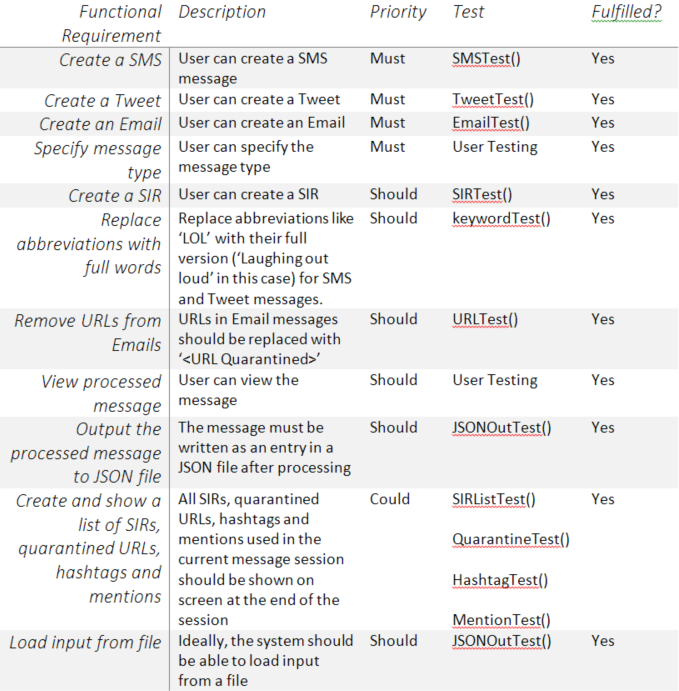
\includegraphics[width=1\textwidth]{funRequirements.PNG}
\caption{\label{fig:funRequirementsTable}The project's functional requirements.}
\end{figure}

\begin{figure}
\centering
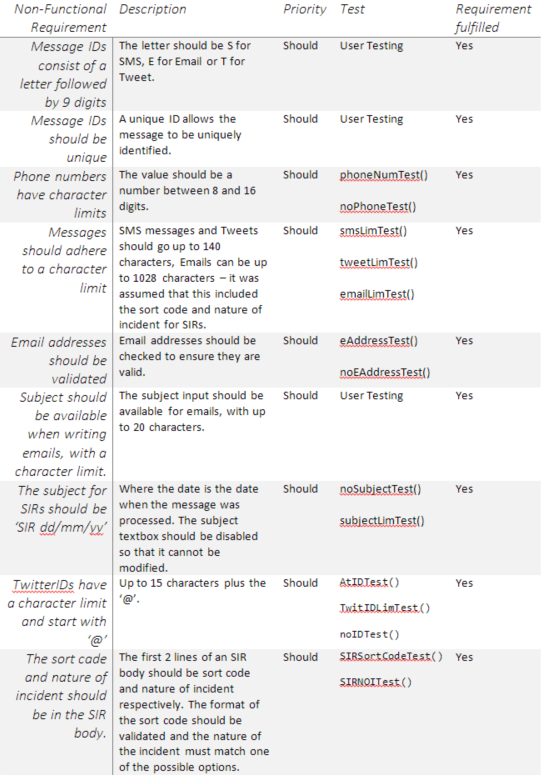
\includegraphics[width=1\textwidth]{noRequirements.PNG}
\caption{\label{fig:noRequirementsTable}The project's non-functional requirements.}
\end{figure}

\begin{figure}
\centering
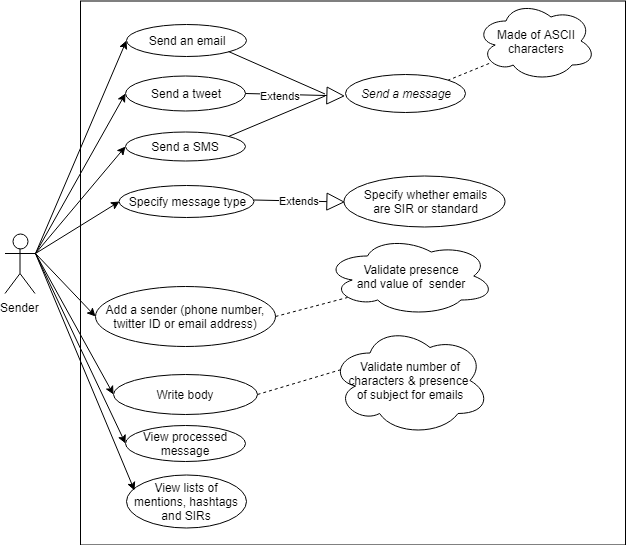
\includegraphics[width=1\textwidth]{UseCaseSET09102Updated2.png}
\caption{\label{fig:usecase}The use case diagram for this project.}
\end{figure}

\begin{figure}
\centering
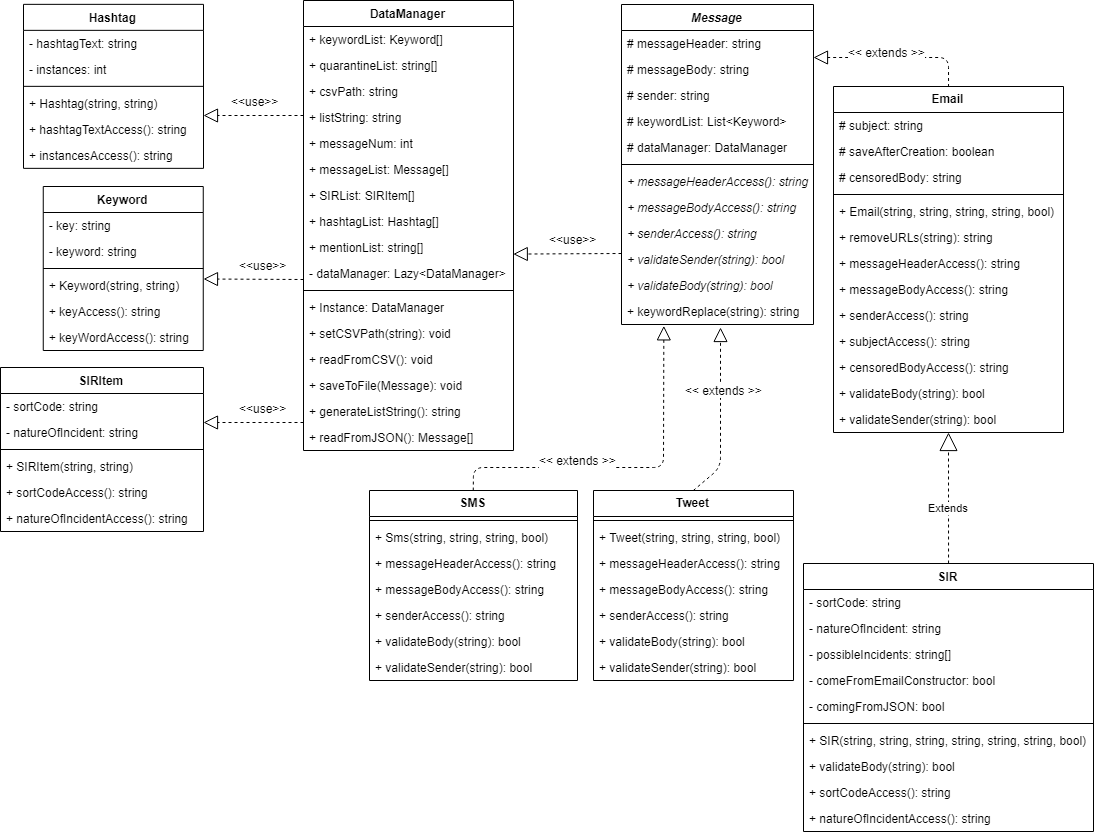
\includegraphics[width=1\textwidth]{ClassDiagramFinal.png}
\caption{\label{fig:class}The class diagram for this project.}
\end{figure}


  
  
\end{thebibliography}
\end{document}